\subsection{Concordia Contracts Migrator} \label{subsection:4-3-3-concordia-contracts-migrator}

\subsubsection{Περιγραφή - Στόχοι υπηρεσίας}

Η υπηρεσία αυτή αποτελείται από ένα εκτελέσιμο πρόγραμμα γραμμής εντολών βασισμένο στο άρθρωμα concordia-contracts, που αναλύθηκε σε προηγούμενη υποενότητα (\ref{subsection:4-3-1-software-units}). Το πρόγραμμα, κατά την εκτέλεσή του, μεταγλωττίζει τα contract και έπειτα τα μεταφορτώνει στο blockchain, το οποίο είναι ορισμένο με χρήση μεταβλητών περιβάλλοντος. Τέλος, αν οι κατάλληλες μεταβλητές περιβάλλοντος είναι ορισμένες, το πρόγραμμα μεταφορτώνει τα τελικά artifact στο αποθετήριο που παρέχει η υπηρεσία Concordia Contracts Provider. Η αρχιτεκτονική της υπηρεσίας Concordia Contracts Migrator φαίνεται στο σχήμα \ref{figure:4-3-concordia-contracts-migrator-architecture}.

\vspace{.5\baselineskip}

\begin{figure}[H]
    \centering
    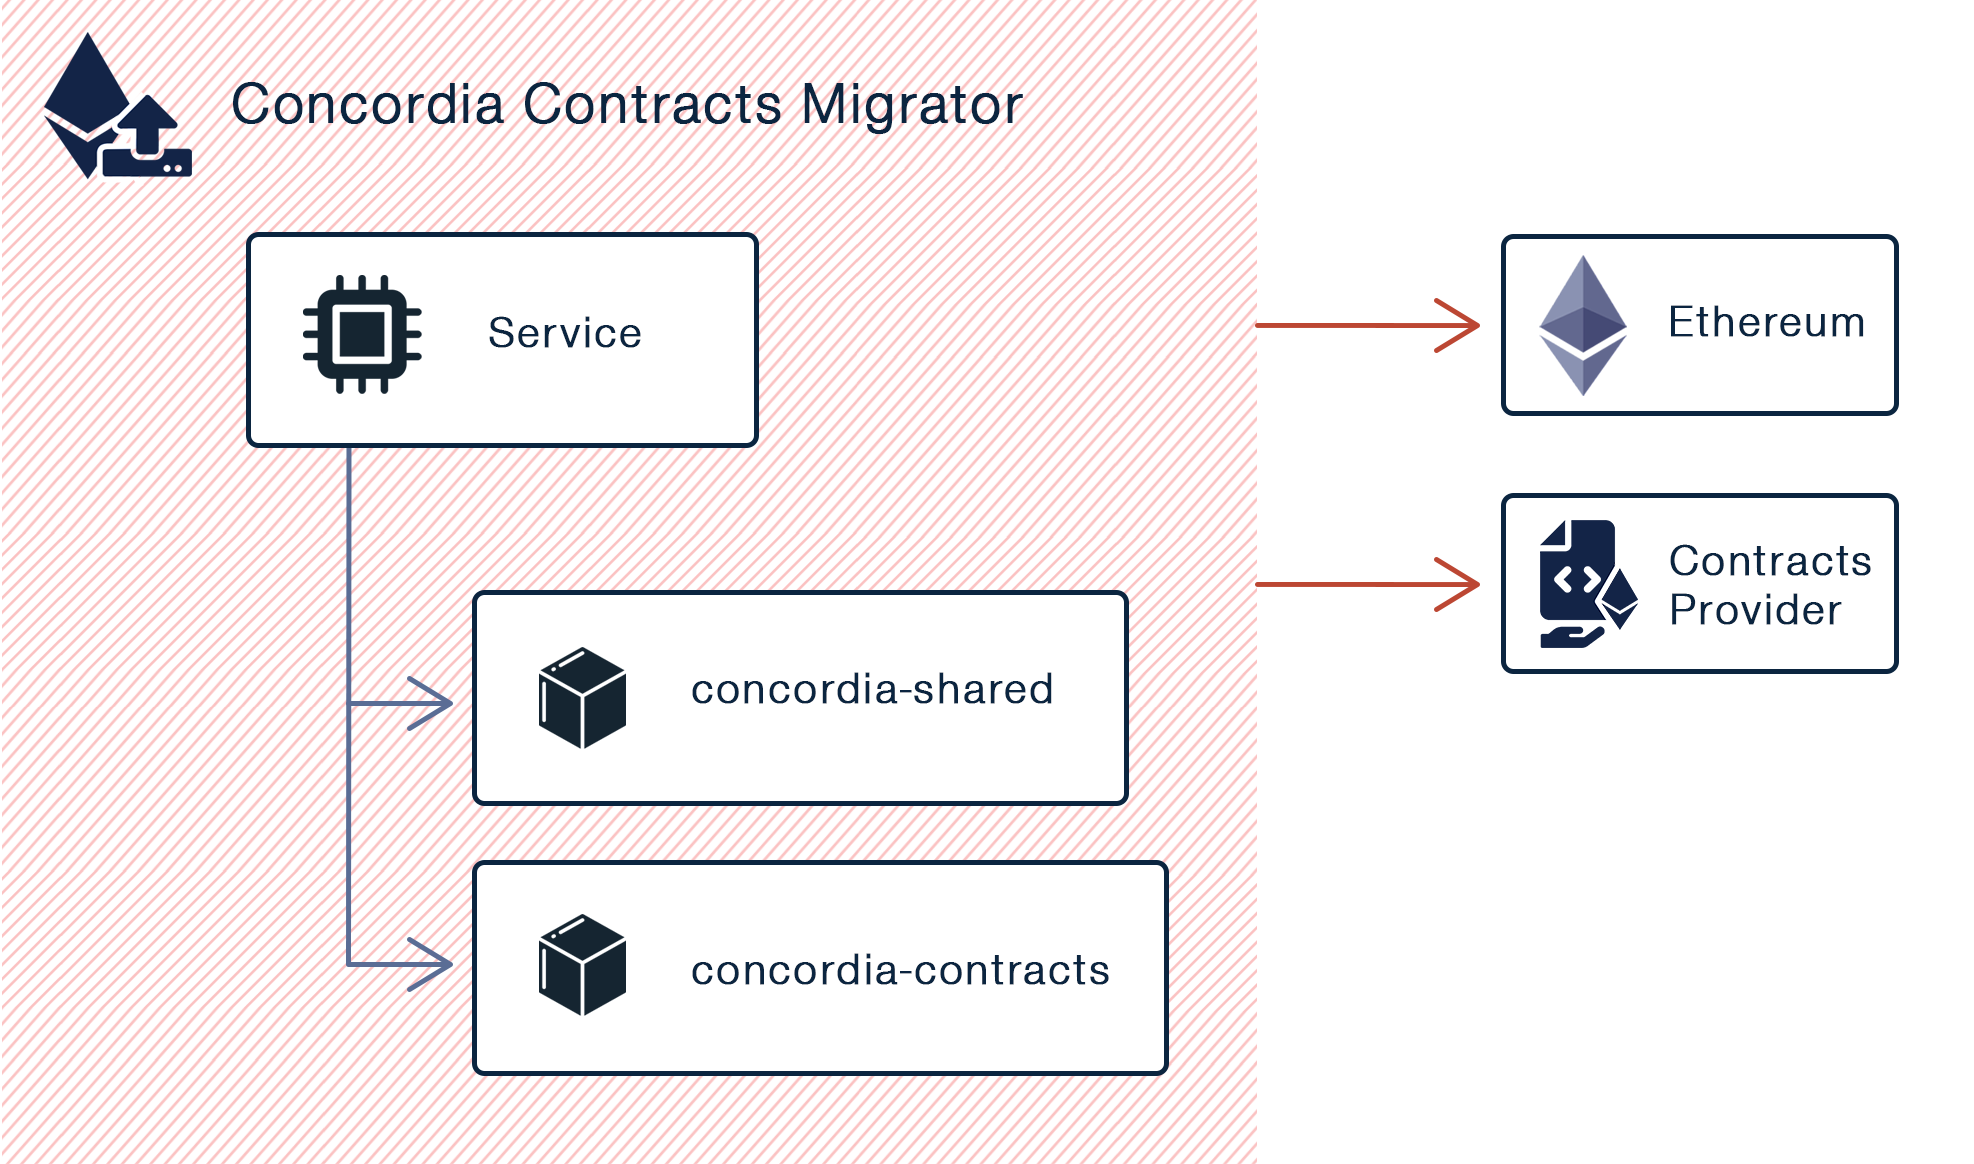
\includegraphics[width=.75\textwidth]{assets/figures/chapter-4/4.3.architecture-4.3.3.concordia-contracts-migrator-architecture.png}
    \caption{Αρχιτεκτονική υπηρεσίας Concordia Contracts Migrator}
    \label{figure:4-3-concordia-contracts-migrator-architecture}
\end{figure}

\subsubsection{Διανομή}

Η υπηρεσία αυτή γίνεται διαθέσιμη για χρήση ως Docker image μέσω του αποθετηρίου εικόνων Docker Hub. Οι χρήστες μπορούν, χρησιμοποιώντας μεταβλητές περιβάλλοντος, να αλλάξουν τη διεύθυνση του blockchain και την τοποθεσία της υπηρεσίας Contracts Provider, στην οποία το πρόγραμμα θα μεταφορτώσει τα contract και τα artifact.